

\section{Introduction} \label{sec:intro}
Image denoising problems consist in estimating an unknown image from a noisy observation in a way that accounts for the underlying uncertainties. Variational and Bayesian methods have become two important approaches for doing so, and in a Bayesian setting these approaches correspond, respectively, to using maximum a posteriori estimators and posterior mean estimators for reconstructing images. The goal of this paper is to describe a broad class of Bayesian posterior mean estimators with quadratic data fidelity term and log-concave prior using Hamilton--Jacobi (HJ) partial differential equations (PDEs) and to use these connections to clarify certain image denoising properties of this class of Bayesian posterior estimators.

To illustrate the main ideas of this paper, we first briefly describe convex finite-dimensional variational and Bayesian methods relevant to image denoising problems. Variational methods formulate image denoising problems as the optimization of a weighted sum of a data fidelity term (which embeds the knowledge of the nature of the noise corrupting the unknown image) and a regularization term (which embeds known properties of the image to reconstruct), where the goal is to minimize this sum to obtain an estimate that hopefully accounts well for both the data fidelity term and the regularization term \cite{chambolle2016introduction,darbon2015convex}. Bayesian methods formulate image denoising problems in a probabilistic framework that combine observed data through a likelihood function (which models the noise corrupting the unknown image) and prior knowledge through a prior distribution (which models known properties of the unknown image) to generate a posterior distribution. An appropriate decision rule that minimizes the posterior expected value of a loss function, also called a Bayes estimator, then selects a meaningful image estimate from the posterior distribution that hopefully accounts well for both the prior knowledge and observed data \cite{demoment1989image,stuart2010inverse,tarantola2005inverse,tikhonov1995numerical,vogel2002computational}. A standard example is the posterior mean estimator, the mean of the posterior distribution, which minimizes the mean squared error (\cite{kay1993fundamentals}, pages 344-345), and more generally, Bregman loss functions~\cite{banerjee2005optimality}.

In this paper, we will focus on the class of finite-dimensional image denoising problems
\begin{equation} \label{eq:image_formation_model}
    \bx = \bu + \boldsymbol{\eta}, %\bx? No matrix A
\end{equation}
where $\bx \in \Rn$ is the observed image, $\bu \in \Rn$ is the unknown image, $\eta$ is independent identically distributed Gaussian noise. This problem is well-known to be ill-posed \cite{aubert2006mathematical,demoment1989image,winkler2003image}, and variational and Bayesian approaches are celebrated methods for solving imaging denoising problems~\cite{aubert2006mathematical,demoment1989image,winkler2003image}. These methods aim to estimate the original uncorrupted image by computing, respectively, the maximum a posteriori (MAP) and posterior mean (PM) estimates
\begin{equation} \label{eq:minimizer_prob}
\bu_{MAP}(\bx,t) \coloneqq \argmin_{\by\in\Rn}\left\{ \frac{1}{2t}\normsq{\bx-\by}+J(\by)\right\}
\end{equation}
and
\begin{equation} \label{eq:pm_estimate}
    \bu_{PM}(\bx,t,\epsilon) \coloneqq \frac{\int_{\Rn} \by e^{-\left(\frac{1}{2t}\normsq{\bx-\by} + J(\by)\right)/\epsilon} \diff\by}{\int_{\Rn} e^{-\left(\frac{1}{2t}\normsq{\bx-\by} + J(\by)\right)/\epsilon} \diff\by}.
\end{equation}
The functions $\by\mapsto \frac{1}{2t}\normsq{\bx-\by}$ and $J\colon\Rn\to\R\cup\{+\infty\}$ in \eqref{eq:minimizer_prob} are, respectively, the (quadratic) data fidelity and regularization terms, and the functions $\by \mapsto e^{-\left(\frac{1}{2t}\normsq{\bx-\by} + J(\by)\right)/\epsilon}$ and $\by \mapsto e^{-J(\by)/\epsilon}$ in \eqref{eq:pm_estimate} are, respectively, the (Gaussian) likelihood function and generalized prior distribution. The parameter $t>0$ controls the relative importance of the data fidelity term over the regularization term, and the parameter $\epsilon$ controls the shape of the posterior distribution in \eqref{eq:pm_estimate}, where small values of $\epsilon$ favor configurations close to the mode, which is the MAP estimate, of the posterior distribution.

Let us illustrate the MAP and PM estimates and their denoising capabilities with an example. We consider an anisotropic versions of the Rudin--Osher--Fatemi (ROF) image denoising model, which consists of considering an anisotropic total variation (TV) regularization term with quadratic data fidelity term \cite{bouman1993generalized,chambolle1997image,rudin1992nonlinear}. Specifically, we define anisotropic TV as follows 
$$
\rm{TV}(\by) = \sum_{i,j\in\{1,\dots n\}} w_{i,j}|y_i - y_j|,
$$
where $w_{i,j} \geqslant 0$ and the value of an image $\by$ at the pixel $i$ is denoted by $y_i \in \R$. For illustration purposes, we assume that a digital image is defined on a two-dimensional regular grid, and only consider the 4-nearest neighbors interactions for defining TV (i.e., $w_{i,j} = w_{j,i} = \frac{1}{2}$  if $i$ and $j$ are neighbors, and $w_{i,j} = w_{j,i} = 0$ otherwise, see~\cite{darbon2006image} for instance). Let $\bx$ denote an observed noisy image and $t$ and $\epsilon$ be parameters as previously defined. Then the associated anisotropic ROF problem \cite{rudin1992nonlinear} takes the form
\begin{equation}\label{eq:rof_model}
\min_{\by \in \Rn}\left\{\frac{1}{2t}\normsq{\bx-\by} + \rm{TV}(\by) \right\}.
\end{equation}
The MAP estimate is the unique minimizer of~\eqref{eq:rof_model},
\begin{equation}\label{eq:rof_model_map}
    \bu_{MAP}(\bx,t) = \argmin_{\by \in \Rn}\left\{\frac{1}{2t}\normsq{\bx-\by} + \rm{TV}(\by) \right\},
\end{equation}
and the PM estimate associated to the anisotropic ROF problem~\eqref{eq:rof_model} is the expected value
\begin{equation}\label{eq:rof_model_pm}
\bu_{PM}(\bx,t,\epsilon) = \frac{\int_{\Rn} \by e^{-\left(\frac{1}{2t}\normsq{\bx-\by} + \rm{TV}(\by)\right)/\epsilon} \diff \by}{\int_{\Rn} e^{-\left(\frac{1}{2t}\normsq{\bx-\by} + \rm{TV}(\by)\right)/\epsilon} \diff\by}.
\end{equation}
We note here that the PM estimate~\eqref{eq:rof_model_pm} with total variation prior and its denoising capabilities were investigated in \cite{louchet2008modeles,louchet2013posterior}. 

Figure~\ref{fig:barbara_images}(a) depicts the image Barbara, which we corrupt with Gaussian noise (zero mean with standard deviation $\sigma = 10$) in Figure~\ref{fig:barbara_images}(b). We let $\bx$ denote this corrupted image, and we choose the parameters $t = 16$ and $\epsilon = 6.25$ in the MAP and PM estimates. The MAP estimate can be computed up to the machine precision using maximum-flow based algorithms \cite{chambolle2009total,darbon2006image,hochbaum2001efficient}, and the PM estimate can be approximated using Markov Chain Monte Carlo methods. Here, we approximated the PM estimate~\eqref{eq:rof_model_pm} using the variable-at-a-time Metropolis--Hastings algorithm with random scan detailed in (\cite{louchet2008modeles}, algorithm 2 on page 42). Specifically, for the parameters of algorithm 2 in \cite{louchet2008modeles}, we used, in the terminology of their algorithm, the parameters $\sigma = 10$ and $\lambda = 32$ (corresponding here to the choice of $t = 16$ and $\epsilon = 6.25$ in~\eqref{eq:rof_model_pm}), we chose the initial point of the algorithm to be the MAP estimate $\bu_{MAP}(\bx,t)$, and finally, we set the internal parameters of algorithm 2 in \cite{louchet2008modeles} as follows: $\alpha = 17.32$ (this values yields an acceptance rate in the algorithm close to the optimal value 0.234 suggested in \cite{roberts2001optimal}), 20,000 for the maximum number of iterations, and $n$ for the subsampling rate.

The MAP and PM estimates associated to the ROF model with these parameters produce the denoised images illustrated in Figures~\ref{fig:barbara_images}(c) and (d). Figures~\ref{fig:zoomed-in_images}(a)-(d) zoom-in on the face of Barbara in Figures~\ref{fig:barbara_images} The denoised image of Barbara with the MAP estimate exhibits staircasing effects \cite{chan2000high,dobson1996recovery,durand2000image} that can be observed in Figure~\ref{fig:zoomed-in_images}(c), whereas the denoised image of Barbara with the posterior mean estimate does not. In either case, the denoised images result in a lost of texture, as can be seen by comparing Figure~\ref{fig:zoomed-in_images}(a) with (c) and (d). 

\begin{figure}[ht]
    \centering
\begin{subfigure}{0.55\textwidth}
    \centering
    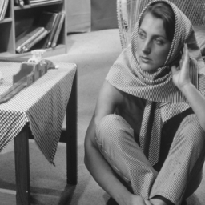
\includegraphics[width = 0.60\textwidth]{barbara_original256x256.png}
    \caption{}
    \label{subfig:barbara_original}
\end{subfigure}%
\begin{subfigure}{0.55\textwidth}
    \centering
    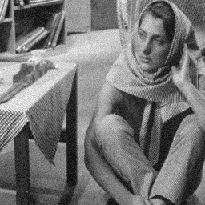
\includegraphics[width = 0.60\textwidth]{barbara_noisy_sigma=10_lambda=32.png}
    \caption{}
    \label{subfig:barbara_noisy}
\end{subfigure}

\begin{subfigure}{0.55\textwidth}
    \centering
    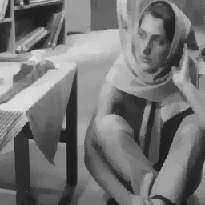
\includegraphics[width = 0.60\textwidth]{barbara_denoised_sigma=10_lambda=32_umap.png}
    \caption{}
    \label{subfig:barbara_umap}
\end{subfigure}%
\begin{subfigure}{0.55\textwidth}
    \centering
    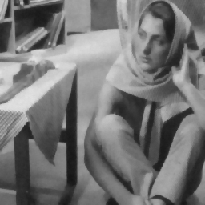
\includegraphics[width = 0.60\textwidth]{barbara_denoised_sigma=10_lambda=32_upm.png}
    \caption{}
    \label{subfig:barbara_upm}
\end{subfigure}
    \caption{The anisotropic ROF model endowed with 4-nearest neighbors is applied to the test image "Barbara". The original image is shown in (a). The image is corrupted by Gaussian noise (zero mean with standard deviation $\sigma = 10$) and is shown in (b). The corresponding minimizer $\bu_{MAP}(\bx,t)$ given by \eqref{eq:rof_model} and posterior mean estimate $\bu_{PM}(\bx,t,\epsilon)$ given by \eqref{eq:rof_model_pm} with parameters $t = 16$ and $\epsilon = 6.25$ are illustrated in (c) and (d), respectively.}
    \label{fig:barbara_images}
\end{figure}

\begin{figure}[ht]
    \centering
\begin{subfigure}{0.55\textwidth}
    \centering
    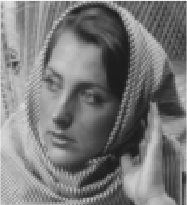
\includegraphics[width = 0.60\textwidth]{barbara_original256x256_zoom-in.png}
    \caption{}
    \label{subfig:barbara_zoom}
\end{subfigure}%
\begin{subfigure}{0.55\textwidth}
    \centering
    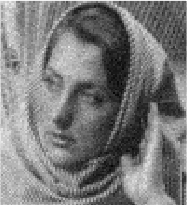
\includegraphics[width = 0.60\textwidth]{barbara_noisy_sigma=10_lambda=32_zoom-in.png}
    \caption{}
    \label{subfig:barbara_noisy_zoom}
\end{subfigure}

\begin{subfigure}{0.55\textwidth}
    \centering
    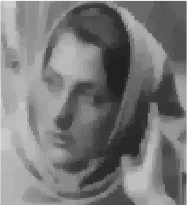
\includegraphics[width = 0.60\textwidth]{barbara_denoised_sigma=10_lambda=32_umap_zoom-in.png}
    \caption{}
    \label{subfig:barbara_umap_zoom}
\end{subfigure}%
\begin{subfigure}{0.55\textwidth}
    \centering
    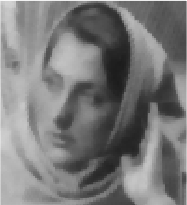
\includegraphics[width = 0.60\textwidth]{barbara_denoised_sigma=10_lambda=32_upm_zoom-in.png}
    \caption{}
    \label{subfig:barbara_upm_zoom}
\end{subfigure}
    \caption{The anisotropic ROF model endowed with 4-nearest neighbors is applied to the test image "Barbara". Images (a)-(d) are zoomed-in versions of the images illustrated in Figure~\ref{fig:barbara_images}.}
    \label{fig:zoomed-in_images}
\end{figure}

Variational methods are popular because the resultant optimization problem for various non-smooth and convex regularization terms used in image denoising problems, such as total variation and $l_1$-norm based regularization terms, is well-understood \cite{bouman1993generalized,candes2006robust,chambolle1997image,darbon2015convex,darbon2019decomposition,donoho2006compressed,rudin1992nonlinear} and can be solved efficiently using robust numerical optimization methods \cite{chambolle2016introduction}. MAP estimates from variational methods are also generally faster to compute than posterior mean estimates, the latter which require complex stochastic methods to compute. Reconstructed images from variational methods with non-smooth and convex regularization terms, however, may have undesirable and visually unpleasant staircasing effects due to the singularities of the non-smooth regularization terms \cite{chan2000high,dobson1996recovery,durand2000image,nikolova2007model,louchet2008modeles,woodford2009global}. This is illustrated for example in Figure 1(c), which contains regions where the pixel values are equal and lead to staircasing effects. In contrast, posterior mean estimates with quadratic fidelity term and total variation regularization terms have been shown to avoid staircasing effects \cite{louchet2008modeles,louchet2013posterior}. This is illustrated for example in Fig.~\ref{fig:barbara_images} and~\ref{fig:zoomed-in_images}(d), where the denoised image with posterior mean estimate does not contain visibly substantial regions where the pixel values are equal.

\bigbreak
\noindent
\textbf{Related work.} 
Several papers have proposed original connections between MAP and Bayesian estimators, including posterior mean estimators. First, \cite{louchet2008modeles,louchet2013posterior} showed that the class of Bayesian posterior mean estimates \eqref{eq:pm_estimate} with TV regularization term $J$ can be expressed as minimizers to optimization problems involving a quadratic fidelity term and a smooth convex regularization term, i.e., there exists a smooth regularization term $f_{\rm{reg}}\colon \Rn \to \R$ such that
\begin{equation}\label{eq:pm_rep_map}
\bu_{PM}(\bx,t,\epsilon) = \argmin_{\by \in \Rn} \left\{\frac{1}{2}\normsq{\bx-\by} + f_{\rm{reg}}(\by)\right\}.
\end{equation}
This result was later extended to general priors \cite{gribonval2011should}, general Gaussian data fidelity terms \cite{gribonval2013reconciling}, and to some non-quadratic data fidelity terms \cite{gribonval2018bayesian,gribonval2018characterization}. To our knowledge, there is no representation formula for this smooth regularization term available in the literature. 

Second, \cite{burger2014maximum} showed that the MAP estimate~\eqref{eq:minimizer_prob} corresponds to a Bayes estimator when the regularization term $J$ is convex and uniformly Lipschitz continuous on $\Rn$, that is, the MAP estimate~\eqref{eq:minimizer_prob} minimizes the posterior expected value of an appropriate loss function. This was later extended by \cite{burger2016bregman} to some log-concave posterior distributions with non-quadratic fidelity term, and later studied from the point of view of differential geometry in \cite{pereyra2019revisiting} and also derived for posterior distributions that are strongly log-concave and at least three times differentiable.

In addition to these results, it is known that under certain assumptions on the regularization term $J$, the value of the minimization problem
\begin{equation} \label{eq:minimization_prob} 
S_{0}(\bx,t)\coloneqq\min_{\by\in\Rn}\left\{ \frac{1}{2t}\normsq{\bx-\by}+J(\by)\right\}
\end{equation}
whose minimizer is the MAP estimate~\eqref{eq:minimizer_prob}, satisfies the first-order HJ PDE 
\begin{equation}
\begin{dcases}
\frac{\partial S_0}{\partial t}(\bx,t)+\frac{1}{2}\normsq{\nabla_{\bx}S_0(\bx,t)}=0 & \mbox{in }\Rn\times(0,+\infty),\\
S_0(\bx,0)=J(\bx) & \mbox{in }\Rn.
\end{dcases}
\end{equation}
The properties of the minimizer $\bu_{MAP}(\bx,t)$ follow from the properties of the solution to this HJ equation~\cite{darbon2015convex,darbon2019decomposition}. In particular, the MAP estimate satisfies the representation formula $\bu_{PM}(\bx,t) = \bx - t\nabla_{\bx}S_0(\bx,t)$. 

We note that the results of \cite{darbon2015convex,darbon2019decomposition} considers only connections between a class of first-order HJ PDEs and MAP estimators. To our knowledge, connections between posterior estimators and HJ PDEs are not available in the literature.

\bigbreak
\noindent
\textbf{Contributions.} 
In this paper, we propose original connections between solutions to HJ PDEs and a broad class of Bayesian methods and posterior mean estimators. These connections are described in Prop.~\ref{thm:visc_hj_eqns} and~\ref{thm:char_opt_sol} for viscous HJ PDEs and first-order HJ PDEs, respectively. We show in Prop.~\ref{thm:visc_hj_eqns} that the posterior mean estimate~\eqref{eq:pm_estimate} is described by the solution to a viscous HJ with initial data corresponding to the convex regularization term $J$, which we characterize in detail in terms of the data $\bx$ and parameters $t$ and $\epsilon$. In particular, the posterior mean estimate~\eqref{eq:pm_estimate} satisfies the representation formula $\bu_{PM}(\bx,t,\epsilon) = \bx - t\nabla_{\bx}S_\epsilon(\bx,t)$. Next, we use the connections between viscous HJ PDEs and posterior mean estimates established in Prop.~\ref{thm:visc_hj_eqns} to show in Prop.~\ref{thm:char_opt_sol} that the posterior mean estimate $\bu_{PM}(\bx,t,\epsilon)$ can be expressed through the gradient of the solution to a first-order HJ PDE with twice continuously differentiable convex initial data $\Rn \ni \bx \mapsto K^{*}_{\epsilon}(\bx,t)-\frac{1}{2}\Vert \bx \Vert_{2}^{2}$, where
\[
K_{\epsilon}(\bx,t) = t\epsilon\ln\left(\frac{1}{(2\pi t\epsilon)^{n/2}}\int_{\dom J}e^{\left(\frac{1}{t}\left\langle \bx,\by\right\rangle -\frac{1}{2t}\left\Vert \by\right\Vert _{2}^{2}-J(\by)\right)/\epsilon}\diff\by\right)
\]
and $\bx \mapsto  K^{*}_{\epsilon}(\bx,t)$ is the Fenchel--Legendre transform of the function $\bx \mapsto K_{\epsilon}(\bx,t)$. In other words, we show
\[
\bu_{PM}(\bx,t,\epsilon) = \argmin_{\by \in \Rn}\left\{\frac{1}{2}\normsq{\bx-\by} + \left( K^{*}_{\epsilon}(\by,t)-\frac{1}{2}\Vert \by \Vert_{2}^{2}\right)\right\}.
\]
This formula gives the representation of the convex regularization term enabling one to express the posterior mean estimate as the minimizer of a convex variational problem, and in fact in terms of the solution to a first-order HJ PDE, thereby extending the results of \cite{louchet2008modeles,gribonval2011should} who showed existence of this regularization term when the data fidelity term is quadratic, but not its representation. The twice continuously differentiability of this regularization term, in particular, implies that the posterior mean estimate $\bu_{PM}(\bx,t,\epsilon)$ avoids image denoising staircasing effects as a consequence of the results derived in (\cite{nikolova2004weakly}, Theorem 3).

We also present several topological properties of posterior mean estimators in Proposition~\ref{prop:topo_properties} and we use these in conjunction with the connections between HJ PDEs and posterior mean estimators to derive representation and monotonicity properties of posterior mean estimators in Propositions~\ref{prop:pm_rep_props} and \ref{prop:mono_properties}, respectively. These properties are then used to derive an optimal upper bound on the mean squared error $\expectationJ{\normsq{\by-\bu_{PM}(\bx,t,\epsilon)}}$, an estimate of the squared difference between the MAP and posterior mean estimates, monotone and non-expansive properties of the posterior mean estimate, and the behavior of the posterior mean estimate $\bu_{PM}(\bx,t,\epsilon)$ in the limit $t \to 0$ (Proposition~\ref{prop:bounds_limits}). Finally, we use the connections between both MAP and posterior mean estimates and HJ PDEs to characterize the MAP estimate~\eqref{eq:minimizer_prob} in the context of Bayesian estimation theory, and specifically in Prop.~\ref{thm:bregman_div} to show that the MAP estimate~\eqref{eq:minimizer_prob} corresponds to the Bayes estimator of the Bayesian risk~\eqref{eq:breg2} whenever $J$ is convex on $\Rn$ and bounded from below. When $J$ is defined only on a strict subset of $\Rn$, we further show that the Bayesian risk~\eqref{eq:breg2} has a corresponding Bayes estimator that is described in terms of the solution to both the first-order HJ PDE~\eqref{thm:e_u_nonvisc_hj} and the viscous HJ PDE~\eqref{thm:visc_hj_eqns}.

\bigbreak
\noindent
\textbf{Organization.} 
In Section \ref{sec:background}, we review concepts of real and convex analysis that will be used throughout this paper. In Section~\ref{sec:connections}, we establish theoretical connections between a broad class of Bayesian posterior mean estimators and HJ PDEs. Our mathematical set-up is described in Subsection~\ref{subsec:set-up}, the connections of posterior mean estimators to viscous HJ PDEs are described in Subsection~\ref{subsec:HJ_eqns_visc}, and the connections of posterior mean estimators to first-order HJ PDEs are described in Subsection~\ref{subsec:HJ_eqns_1order}. We use these connections to establish various properties of posterior mean estimators in Section~\ref{sec:properties_estimators}. Specifically, we present topological, representation, and monotonicity properties of posterior mean estimators in Subsection~\ref{subsec:prop_topo-rep-mono}, an optimal upper bound on the mean squared error $\expectationJ{\normsq{\by-\bu_{PM}(\bx,t,\epsilon)}}$, an estimate of the squared difference between the MAP and posterior mean estimates, monotone and non-expansive properties of the posterior mean estimate, and the behavior of the posterior mean estimate $\bu_{PM}(\bx,t,\epsilon)$ in the limit $t \to 0$ in Subsection~\ref{subsec:prop_bounds-est}. Finally, we establish properties of MAP and posterior mean estimators in terms of Bayesian risks involving Bregman divergences in Subsection~\ref{subsec:prop_breg_div}.